% \chapter{Υλοποίηση}
% Στο προηγούμενο κεφάλαιο φάνηκε αναλυτικά πως τα δεδομένα του \en{dataset} έφτασαν μέσω των διαφόρων διεργασιών της προεπεξεργασίας σε μια πιο ποιοτική και καθαρή μορφή. Για να φανεί χρήσιμη η πληροφορία αυτή, χρειάζεται το αδόμητο κείμενο να μετατραπεί σε κάποια κατανοητή μορφή για τους υπολογιστές, όπως πίνακες ή διανύσματα από χαρακτηριστικά (features).

% Αυτό γίνεται με χρήση της μεθόδου \en{tf-idf}, ο τρόπος λειτουργίας της οποίας αναλύθηκε σε προηγούμενο κεφάλαιο. 

% Έπειτα, το Σχήμα~ \ref{figure5.1} εμφανίζει την απεικόνιση του πίνακα που προέκυψε από την \en{tf-idf} με χρήση της μεθόδου \en{t-SNE} όπου γίνεται εμφανές πως πολλές κατηγορίες-ειδικότητες αλληλοκαλύπτονται.

% \begin{figure} [ht!]
% \centering
% 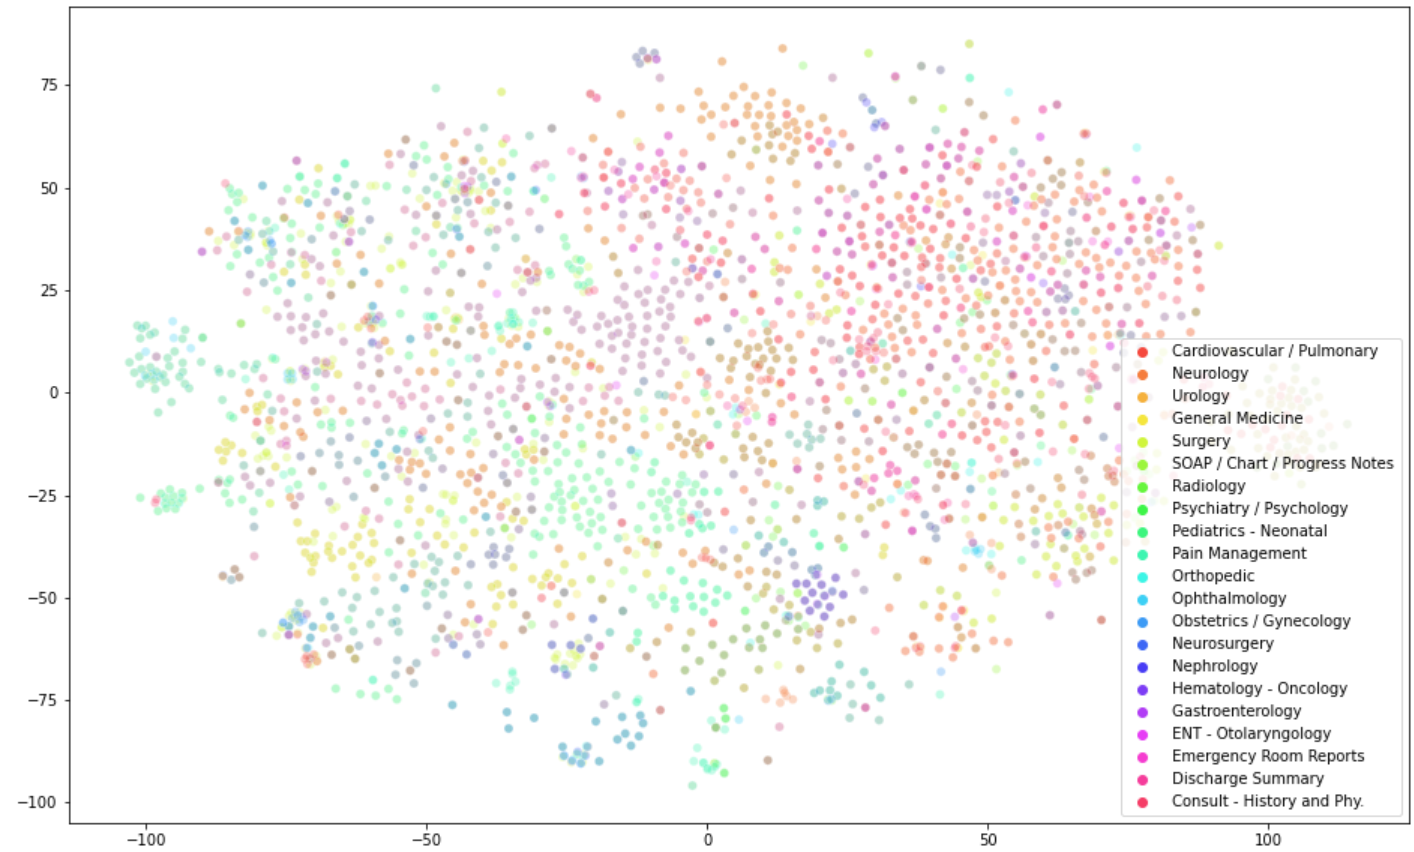
\includegraphics[width=\textwidth,height=20cm,keepaspectratio]{pictures/5.1tsne.png} 
% \caption{Η γραφική απεικόνιση του αλγορίθμου \en{t-SNE}}\label{figure5.1}
% \end{figure}

% Στη συνέχεια εφαρμόζεται η μέθοδος \en{PCA} στον πίνακα \en{tf-idf} με στόχο τη μείωση διαστατικότητας. 

% Η \en{Sklearn (ή Scikit-learn)} είναι μια βιβλιοθήκη της \en{Python} η οποία προσφέρει διάφορες δυνατότητες για επεξεργασία δεδομένων και χρησιμοποιείται συνήθως για ταξινόμηση, ομαδοποίηση και επιλογή μοντέλου. 

% Για να εκπαιδεύσουμε το μοντέλο χρησιμοποιώντας ένα συγκεκριμένο \en{dataset} θα πρέπει να το «τεστάρουμε» πάνω σε ένα δεύτερο \en{dataset}. Όταν έχουμε μόνο ένα, όπως στη δική μας περίπτωση, το χωρίζουμε στα δύο χρησιμοποιώντας τη μέθοδο \en{train\_test\_split()} της \en{sklearn}. 
% Η μέθοδος αυτή χωρίζει το σύνολο των \en{data arrays} σε δύο υποσύνολα: \en{training set} (Σύνολο εκπαίδευσης) και \en{test set} (Σύνολο αξιολόγησης). 

% Έτσι, μετά την εφαρμογή του διαχωρισμού έχουμε:
% \begin{itemize}
%     \item \en{Train\_Set\_Size: (3447, 587) }
%     \item \en{Test\_Set\_Size: (1150, 587) }
% \end{itemize}


% Στη συνέχεια, εφαρμόζουμε στα δεδομένα Λογιστική Παλινδρόμηση \en{(Logistic Regression)} για να εκπαιδεύσουμε το μοντέλο στα \en{training data} και να κάνει την πρόβλεψη στα \en{test data}.
% Η εφαρμογή της λογιστικής παλινδρόμησης στη βιβλιοθήκη της \en{Python} \en{scikit-learn} μπορεί να προσεγγιστεί από την κλάση \en{LogisticRegression}. 


% Μετά απο αυτήν τη διαδικασία κατασκευάζουμε τον πίνακα σύγχυσης (\en{confusion matrix}). 
% Πρόκειται για έναν \en{MxM} πίνακα, όπου το \en{(i,j)} στοιχείο του ισούται με το πλήθος των σημείων που, ενώ προέρχονται από την κλάση \en{i}, καταχωρούνται στην κλάση \en{j}. 
% Δίνει πληροφορίες σχετικά με το αν κάποιες κλάσεις έχουν την τάση να συγχέονται με άλλες κλάσεις.

% Από τη γραφική απεικόνιση του πίνακα σύγχυσης που φαίνεται στο Σχήμα~ \ref{figure5.3}, παρατηρούμε πως μεγαλύτερη σύγχυση υπάρχει σε συγκεκριμένες ειδικότητες όπως η χειρουργική, οι οποίες έχουν την ιδιότητα υπερκλάσης, αφού επικαλύπτονται με άλλες ειδικότητες εκ φύσεως.

% \begin{figure} [ht!]
% \centering
% 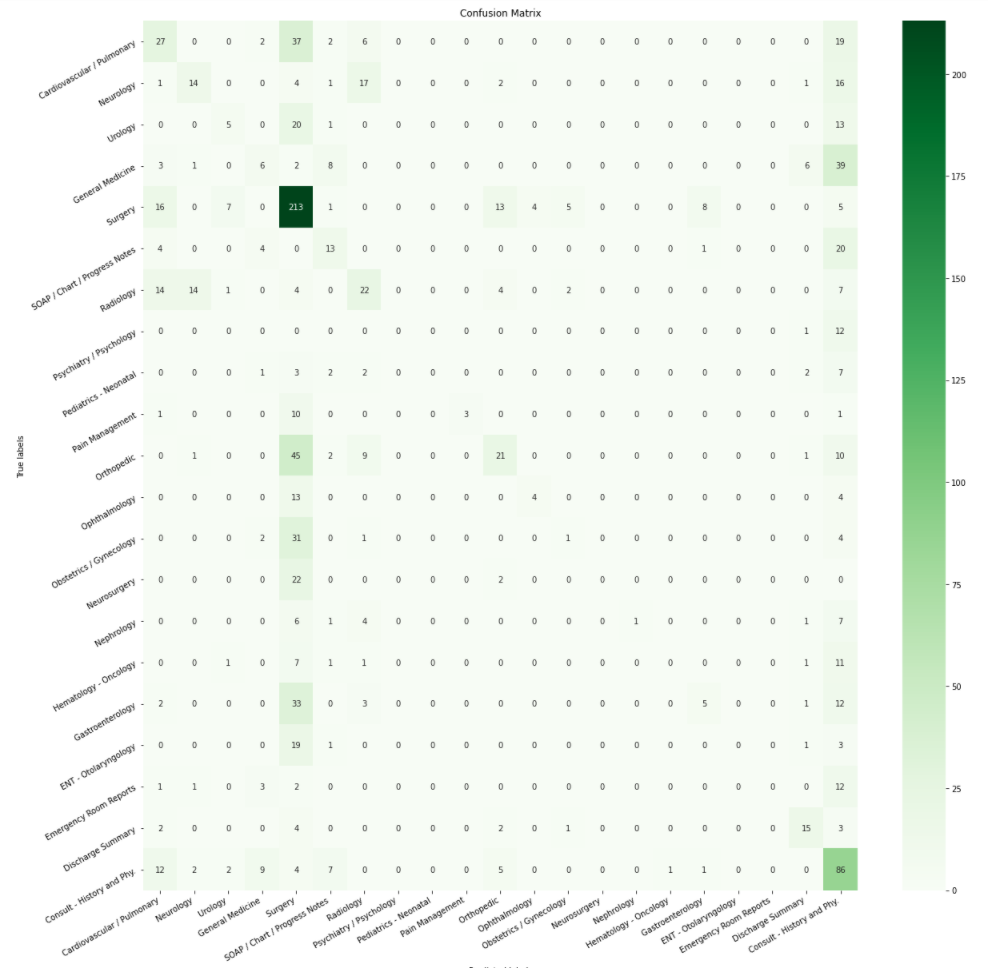
\includegraphics[width=\textwidth,height=20cm,keepaspectratio]{pictures/5.3cMatrix.png} 
% \caption{Η γραφική απεικόνιση του πίνακα σύγχυσης}\label{figure5.3}
% \end{figure}
% \clearpage

% H βιβλιοθήκη \en{sklearn} προσφέρει τη μέθοδο \en{classification\_report()} η οποία τυπώνει τις εκτιμήσεις διαφόρων μετρικών πάνω στην ποιότητα  των αποτελεσμάτων πρόβλεψεις του αλγορίθμου. 

% Οι μετρικές αυτές είναι:
% \begin{enumerate}
%     \item Ορθότητα (\en{Accuracy)}
%     \item Ανάκληση (\en{Recall)} 
%     \item Ακρίβεια (\en{Precision)} 
%     \item \en{F-Measure} 
% \end{enumerate}

% Τα πρώτα αποτελέσματα ακρίβειας ταξινόμησης ανά κατηγορία φαίνονται στον παρακάτω πίνακα (Σχήμα ~\ref{figure5.4}:
 
% \begin{figure} [ht!]
% \centering
% 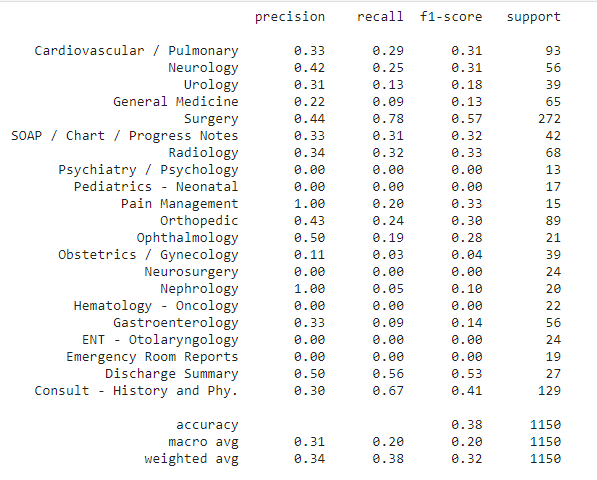
\includegraphics[width=\textwidth,height=20cm,keepaspectratio]{pictures/5.4results.png} 
% \caption{Πίνακας πρώτων αποτελεσμάτων μετρικών ταξινόμησης}\label{figure5.4}
% \end{figure}
% \clearpage

% Από το \en{classification report} παρατηρούμε ότι τα αποτελέσματα ακρίβειας είναι αρκετά χαμηλά. Αυτό οφείλεται στο οτι πολλές απο τις κατηγορίες αλληλοεπικαλύπτονται, όπως φαίνεται και στον πίνακα σύγχυσης. Επειδή αυτό συμβαίνει λόγω της φύσης των δεδομένων, καθώς σε κάποια περιστατικά δε γίνεται να αποφανθεί οτι εμπίπτουν μόνο σε μια συγκεκριμένη ιατρική ειδικότητα, στο επόμενο βήμα αφαιρούνται απο το σύνολο των δεδομένων οι ειδικότητες που δημιουργούν αυτόν το «θόρυβο».

% Οι ειδικότητες που απαλείφονται είναι: 
% \begin{enumerate}
%     \en{\item Surgery
%         \item SOAP / Chart / Progress Notes
%         \item Consult - History and Phy.
%         \item Emergency Room Reports
%         \item Discharge Summary
%         \item Pain Management
%         \item General Medicine}
% \end{enumerate}


% Επίσης, λόγω κοινού γνωστικού πεδίου, συγχωνεύονται οι εξής κατηγορίες:
% \begin{enumerate}
%     \en{\item Neurosurgery \& Neurology
%         \item Nephrology \& Urology}
% \end{enumerate}

% Ο πίνακας του πλήθους εγγραφών ανα κατηγορία μετά τη διαμόρφωση του έχει τη μορφή που παρουσιάζεται στο Σχήμα ~\ref{figure5.5}:
% \begin{figure} [ht!]
% \centering
% 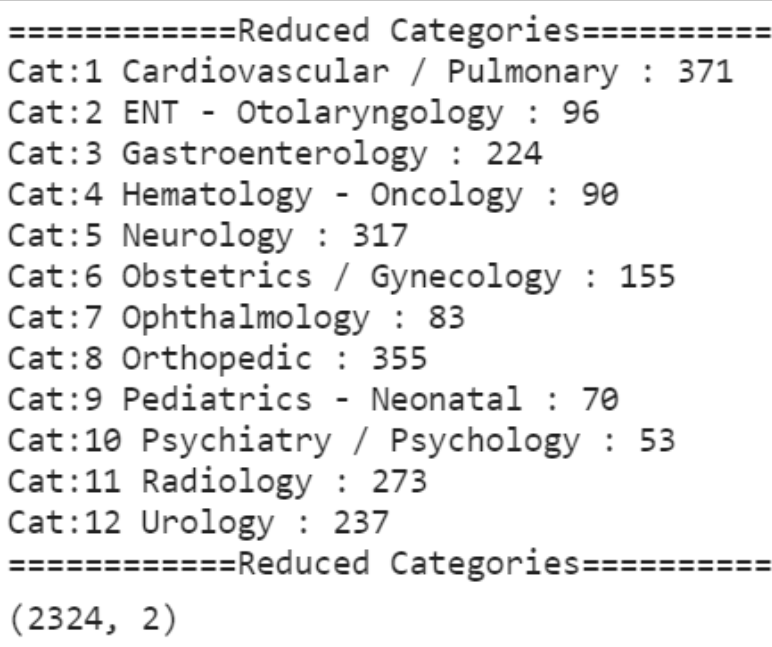
\includegraphics[width=\textwidth,height=7cm,keepaspectratio]{pictures/5.4reducedCat(12cat).png} 
% \caption{Το πλήθος εγγραφών ανά κατηγορία μετά την απαλοιφή και τη συγχώνευση κάποιων κατηγοριών}\label{figure5.5}
% \end{figure}


% Το \en{sciSpacy} είναι ένα πακέτο της  \en{Python} το οποίο περιέχει τα μοντέλα  \en{Spacy} και είναι σχεδιασμένο για προεπεξεργασία σε κείμενα που περιέχουν οντότητες που αποτελούν ιατρική, επιστημονική ή κλινική ορολογία.

% Αξιοποιώντας τη δυνατότητα αυτού του πακέτου, δημιουργείται η συνάρτηση \en{process\_text()} η οποία περνάει κάθε εγγραφή του πεδίου \en{transcription} ως είσοδο στη μέθοδο \en{nlp()} του μοντέλου \en{en\_ner\_bionlp13cg\_md} του πακέτου \en{sciSpacy}, η οποία επιστρέφει το σύνολο λέξεων που έχουν ιατρική, επιστημονική ή κλινική νοηματική αξία.


% Έπειτα, εφαρμόζουμε αναδρομικά όλη τη διαδικασία:
% \begin{enumerate}
%     \item Προεπεξεργασία (εφαρμογή \en{sciSpacy})
%     \item \en{Tf-Idf} αξιολόγηση
%     \item Απεικόνιση του πίνακα \en{Tf-Idf} με χρήση της μεθόδου \en{t-SNE}
%     \item Εφαρμογή \en{PCA} στον πίνακα \en{Tf-Idf}
%     \item Εκ νέου διαχωρισμός δεδομένων σε \en{training set} και \en{test set}
%     \item Εφαρμογή λογιστικής παλινδρόμησης \en{(logistic regression)}
%     \item Κατασκευή Πίνακα Σύγχυσης \en{(confusion matrix)}
%     \item Εμφάνιση νέων αποτελεσμάτων μετρικών ποιότητας πρόβλεψης
% \end{enumerate}

% Το Σχήμα~ \ref{figure5.6} εμφανίζει την απεικόνιση του πίνακα που προέκυψε από την \en{tf-idf} με χρήση της μεθόδου \en{t-SNE} μετά την εκ νέου προεπεξεργασία των δεδομένων 

% \begin{figure} [ht!]
% \centering
% 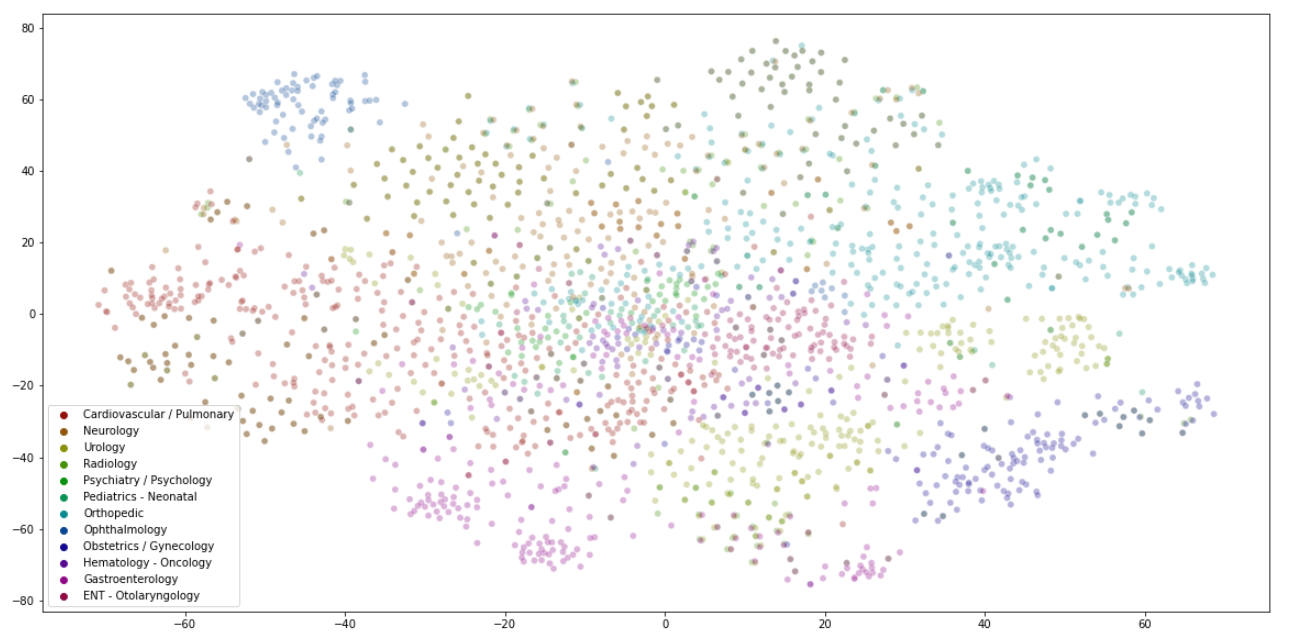
\includegraphics[width=\textwidth,height=12cm,keepaspectratio]{pictures/5.6tsne2.png} 
% \caption{Η νέα γραφική απεικόνιση του αλγορίθμου \en{t-SNE}}\label{figure5.6}
% \end{figure}


% Ο νέος Πίνακας Σύγχυσης και ο νέος Πίνακας αποτελεσμάτων μετρικών ταξινόμησης φαίνονται στα σχήματα ~\ref{figure5.7} και ~\ref{figure5.8}

% \begin{figure} [ht!]
% \centering
% 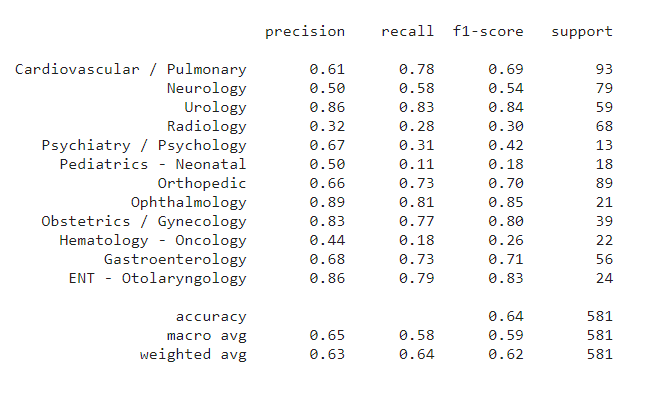
\includegraphics[width=\textwidth,height=8cm,keepaspectratio]{pictures/5.8results2.png} 
% \caption{Πίνακας Αποτελεσμάτων μετρικών ταξινόμησης μετά την επεξεργασία με το πακέτο \en{sciSpacy}}\label{figure5.8}
% \end{figure}

% \begin{figure} [ht!]
% \centering
% 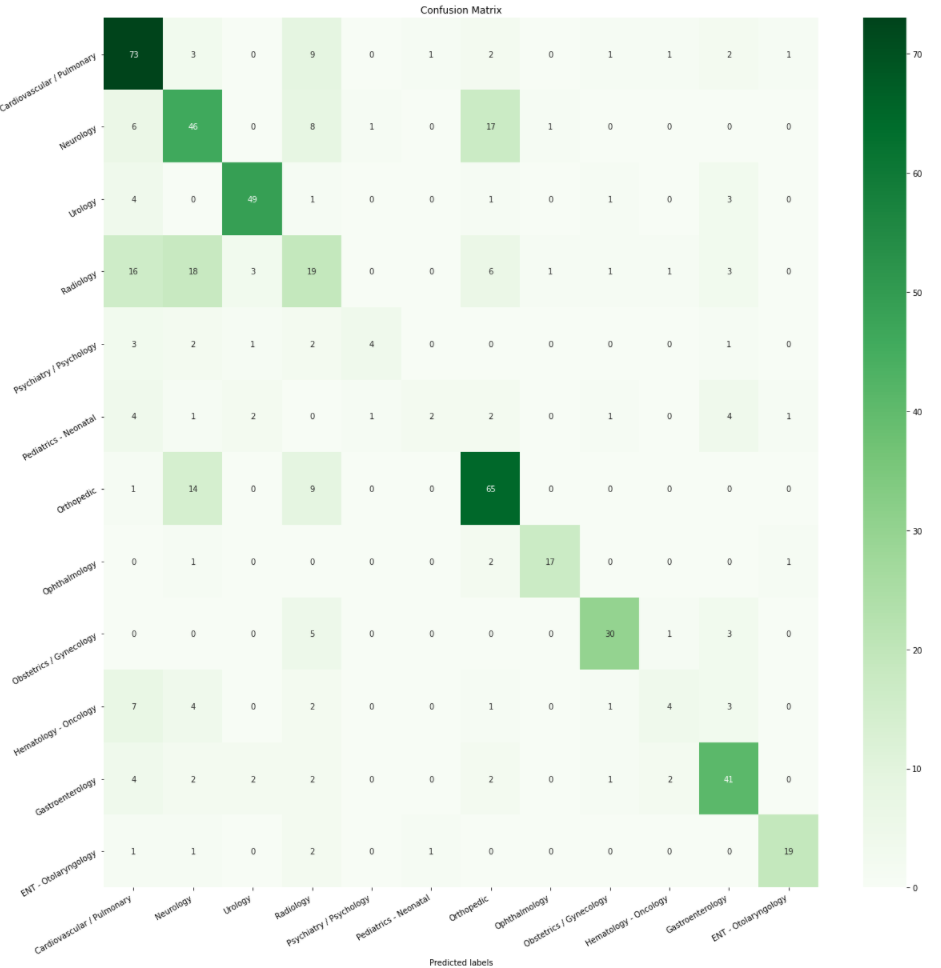
\includegraphics[width=\textwidth,height=12cm,keepaspectratio]{pictures/5.7cMatrix2.png} 
% \caption{Πίνακας Σύγχυσης  μετά την επεξεργασία με το πακέτο \en{sciSpacy}}\label{figure5.7}
% \end{figure}
% \clearpage

% Παρατηρούμε εμφανώς βελτιωμένα αποτελέσματα στα \en{scores} των διάφορων μετρικών. (προηγούμενα αποτελέσματα στο σχήμα ~\ref{figure5.4})
% Παρ’ όλα αυτά, εξακολουθεί να υπάρχει ανισορροπία στο πλήθος των υπαρχόντων δεδομένων μεταξύ των κατηγοριών. 

% Στα πλαίσια της συγκεκριμένης εργασίας ακολουθήθηκαν σε προηγούμενα βήματα και οι δύο προσεγγίσεις αντιμετώπισης της ανισορροπίας των δεδομένων \en{(oversampling} και \en{undersampling}: αφαιρέθηκαν οι κλάσεις που αποτελούσαν μειονότητες καθώς και η κλάση της χειρουρικής που περιείχε δεδομένα κατά πολύ μεγαλύτερα σε όγκο σε σχέση με τις υπόλοιπες κλάσεις τα οποία επίσης συγχέονταν με αυτές λόγω επικαλυπτόμενων γνωστικών πεδίων.

% Μία ακόμα απλή προσέγγιση για την αντιμετώπιση του προβλήματος θα ήταν να χρησιμοποιηθεί η απλούστερη \en{oversampling} τεχνική η οποία υποδεικνύει τη δημιουργία διπλότυπων στιγμιοτύπων στις κατηγορίες που αποτελούν μειονότητες. Κάτι τέτοιο όμως, παρ' ότι φαινομενικά επιφέρει μεγαλύτερη ισορροπία στα δεδομένα, δεν προσθέτει καμία καινούρια πληροφορία στο μοντέλο εκπαίδευσης.

% Γι' αυτό θα χρησιμοποιηθεί η τεχνική \en{SMOTE (Synthetic Minority Oversampling Technique)}.


% Πριν τη δημιουργία νέου \en{dataset} με την τεχνική \en{SMOTE} τα δεδομένα ήταν τα εξής:
% \en{
% \begin{itemize}
%     \item Train\_Set\_Size: (1743, 696)
%     \item Test\_Set\_Size: (581, 696) 
% \end{itemize}}


% Μετά τη δημιουργία νέου \en{dataset} με την τεχνική \en{SMOTE} τα δεδομένα είναι τα εξής:
% \en{
% \begin{itemize}
%     \item Train\_Set\_Size: (1981, 696)
%     \item Test\_Set\_Size: (661, 696) 
% \end{itemize}
% }

% \clearpage 
% \section{Λογιστική Παλινδρόμηση }

% Στη συνέχεια γίνεται εφαρμογή Λογιστικής Παλινδρόμησης και παράγεται ο νέος Πίνακας Σύγχυσης (Σχήμα ~ \ref{figure5.10}):

% \begin{figure} [ht!]
% \centering
% 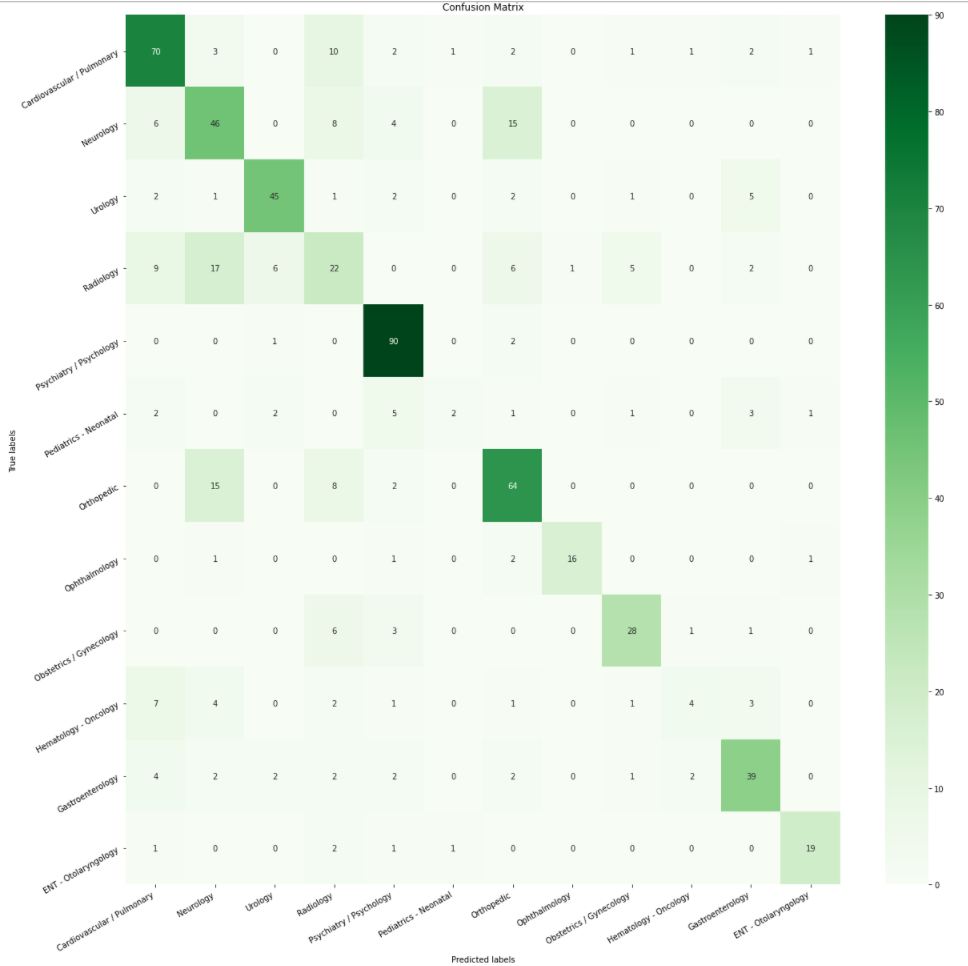
\includegraphics[width=\textwidth,height=12cm,keepaspectratio]{pictures/5.10CMatrix3.png} 
% \caption{Πίνακας Σύγχυσης μετά την εφαρμογή της τεχνικής \en{SMOTE}}\label{figure5.10}
% \end{figure}

% \clearpage
% Τέλος, δημιουργείται ο πίνακας των τελικών αποτελεσμάτων μετρικών ταξινόμησης ο οποίος φαίνεται στο σχήμα ~\ref{figure5.11}.

% \begin{figure} [ht!]
% \centering
% 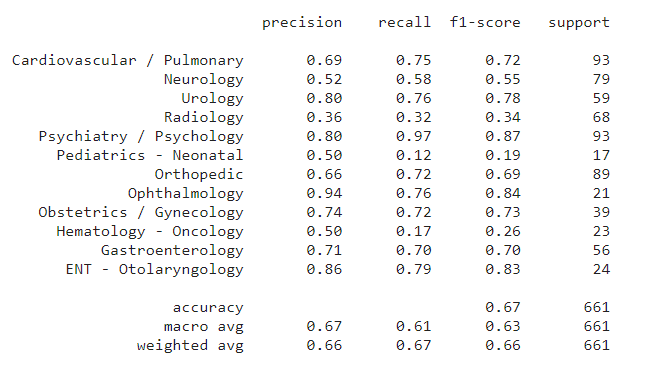
\includegraphics[width=\textwidth,height=8cm,keepaspectratio]{pictures/5.11results3.png} 
% \caption{\en{Logistic Regression: }Πίνακας τελικών Αποτελεσμάτων μετρικών ταξινόμησης μετά την εφαρμογή της τεχνικής \en{SMOTE}}\label{figure5.11}
% \end{figure}

% Τα τελικά αποτελέσματα είναι εμφανώς βελτιωμένα. 
% Παρατηρούμε οτι σε συγκεκριμένες κατηγορίες όπως \en{Neurology, Radiology} και \en{Hematology} τα αποτελέσματα ταξινόμησης παραμένουν χαμηλά καθώς οι περιγραφές των περιστατικών εξακολουθούν να αφορούν παραπάνω απο μία ειδικότητες. 


% Στη συνέχεια, για την ταξινόμηση του κειμένου, δοκιμάζεται η επίδοση των αλγορίθμων:
% \begin{enumerate}
%     \item \en{Naïve Bayes} 
%     \item \en{SVM}
%     \item \en{kNN}
% \end{enumerate}


% διατηρώντας ως είσοδο το \en{dataset} στην τελευταία μορφή που ταξινομήθηκε με τη μέθοδο της λογιστικής παλινδρόμησης, πριν την επεξεργασία για επίτευξη \en{oversampling} με την τεχνική \en{SMOTE}.

% \clearpage
% \section{Αλγόριθμος \en{Naïve Bayes}}
% Ο πίνακας αποτελεσμάτων των μετρικών ταξινόμησης που παράγεται από τη μέθοδο \en{classification\_report()} για τον Αλγόριθμο \en{Naïve Bayes} φαίνεται στο σχήμα ~\ref{figure5.12}.

% \begin{figure} [ht!]
% \centering
% 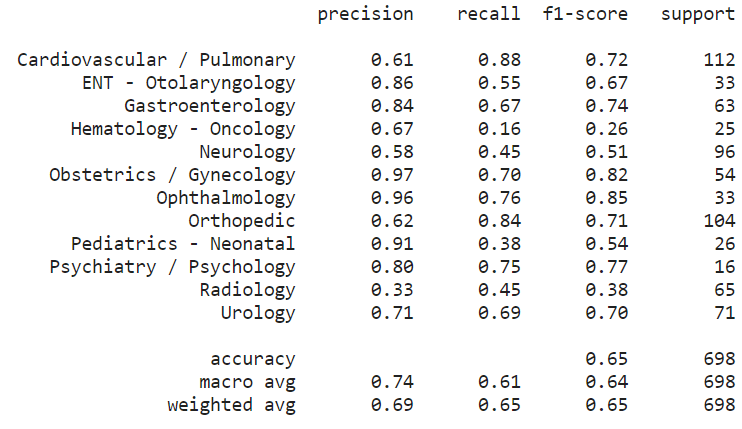
\includegraphics[width=\textwidth,height=8cm,keepaspectratio]{pictures/NAiveBAyes_NO_SMOTE.png} 
% \caption{\en{Naïve Bayes: }Πίνακας Αποτελεσμάτων μετρικών ταξινόμησης}\label{figure5.12}
% \end{figure}
% \clearpage

% \section{Αλγόριθμος \en{SVM}}

% Ο πίνακας αποτελεσμάτων των μετρικών ταξινόμησης που παράγεται από τη μέθοδο \en{classification\_report()} για τον Αλγόριθμο \en{SVM} φαίνεται στο σχήμα ~\ref{figure5.13}.

% \begin{figure} [ht!]
% \centering
% 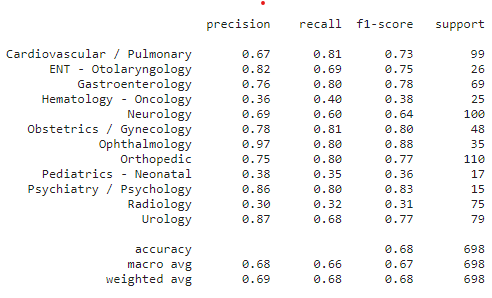
\includegraphics[width=\textwidth,height=8cm,keepaspectratio]{pictures/SVM_NO_SMOTE.png} 
% \caption{\en{SVM: }Πίνακας Αποτελεσμάτων μετρικών ταξινόμησης}\label{figure5.13}
% \end{figure}
% \clearpage

% \section{Αλγόριθμος \en{kNN}}
% Ο πίνακας αποτελεσμάτων των μετρικών ταξινόμησης που παράγεται από τη μέθοδο \en{classification\_report()} για τον Αλγόριθμο \en{kNN} φαίνεται στο σχήμα ~\ref{figure5.14}.

% \begin{figure} [ht!]
% \centering
% 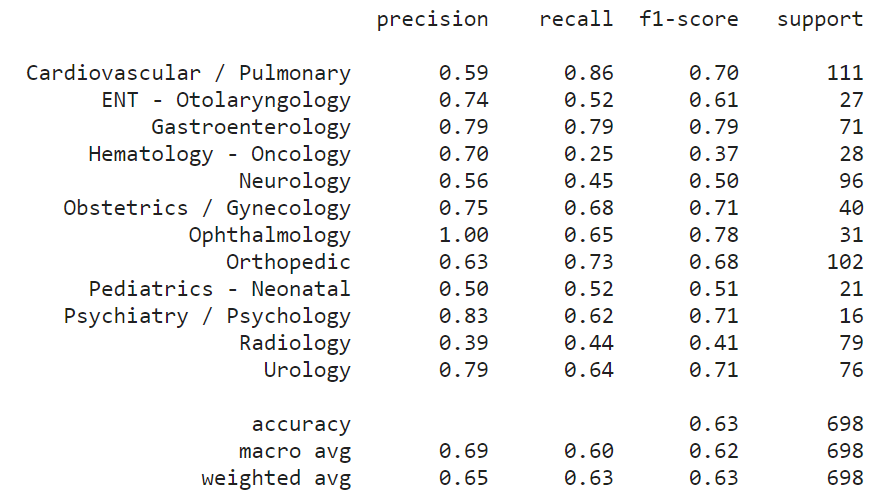
\includegraphics[width=\textwidth,height=8cm,keepaspectratio]{pictures/knn_NO_SMOTE.png} 
% \caption{\en{kNN: }Πίνακας Αποτελεσμάτων μετρικών ταξινόμησης}\label{figure5.14}
% \end{figure}




% \section{\en{Word2Vec - Neural Network}}




